% Methode partie 1

\begin{frame}{La différenciation retardée}
\begin{itemize}
\item<1-> Blocs de 30*30 standards 
\item<2-> Pieds standards
\item<3-> Peinture / Lasure
\item<4-> Revêtement thermique
\item<5-> Trou 
\end{itemize}
\end{frame}

\begin{frame}{Nomenclature}
	\begin{figure}[H]
\centering
\includegraphics[scale=0.4]{../Methodes/captures/Bloc_base.PNG}
\caption{Nomenclature du bloc}
	\end{figure}		
\end{frame}

\begin{frame}{Nomenclature}
	\begin{figure}[H]
\centering
\includegraphics[scale=0.4]{../Methodes/captures/Pieds.PNG}
\caption{Nomenclature du pied}
	\end{figure}		
\end{frame}

\begin{frame}{Procédés}
	\begin{figure}[H]
\centering
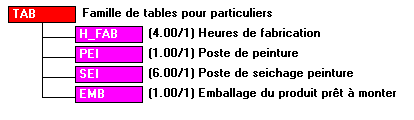
\includegraphics[scale=0.4]{../Methodes/captures/procede_fab_table_particulier.PNG}
\caption{Procédé}
	\end{figure}		
\end{frame}
